\documentclass[tikz,border=6pt]{standalone}
\usepackage{tikz}
\usetikzlibrary{arrows.meta,positioning,shapes.geometric}
\definecolor{nebula}{HTML}{6366F1}
\definecolor{spark}{HTML}{14B8A6}
\definecolor{ink}{HTML}{334155}
\begin{document}
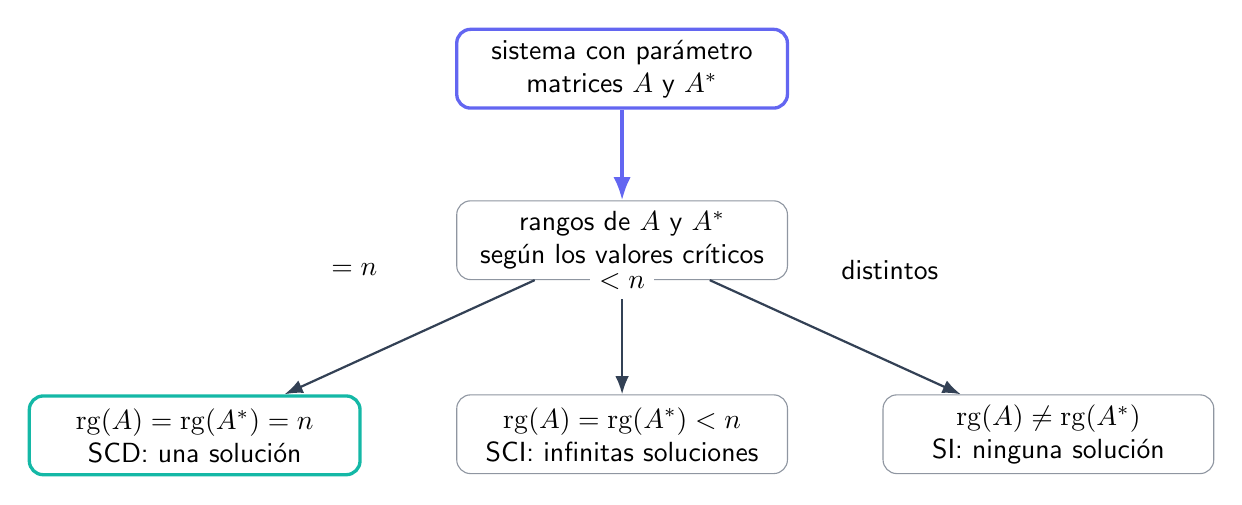
\begin{tikzpicture}[font=\sffamily,>=Latex,node distance=1.15cm,box/.style={draw=ink!55,rounded corners=5pt,minimum width=4.2cm,minimum height=1cm,align=center,fill=white}]
  \node[box,draw=nebula,very thick] (start) {sistema con par\'ametro\\matrices $A$ y $A^*$};
  \node[box,below=of start] (ranks) {rangos de $A$ y $A^*$\\seg\'un los valores cr\'iticos};
  \node[box,below left=1.45cm and 1.2cm of ranks,draw=spark,very thick] (equaln) {$\mathrm{rg}(A)=\mathrm{rg}(A^*)=n$\\SCD: una soluci\'on};
  \node[box,below=1.45cm of ranks] (equallow) {$\mathrm{rg}(A)=\mathrm{rg}(A^*)<n$\\SCI: infinitas soluciones};
  \node[box,below right=1.45cm and 1.2cm of ranks] (different) {$\mathrm{rg}(A)\ne\mathrm{rg}(A^*)$\\SI: ninguna soluci\'on};
  \draw[->,very thick,nebula] (start)--(ranks);
  \draw[->,thick,ink] (ranks)--(equaln);
  \draw[->,thick,ink] (ranks)--(equallow);
  \draw[->,thick,ink] (ranks)--(different);
  \node[fill=white] at (-3.4,-2.55) {$=n$};
  \node[fill=white] at (0,-2.7) {$<n$};
  \node[fill=white] at (3.4,-2.55) {distintos};
\end{tikzpicture}
\end{document}
